% JUMP TO LINE 60, 75
\documentclass{article}
\usepackage[letterpaper,portrait,top=0.4in, left=0.6in, right=0.6in, bottom=1in]{geometry}

\usepackage{amsmath, amsfonts, amsthm, amssymb}
\usepackage{graphicx, float}
\usepackage{suffix}
\usepackage{multicol}
\usepackage{cancel}
\usepackage{mdframed}
\usepackage{mathtools}
\usepackage{tcolorbox}
\usepackage{hyperref}
\usepackage[per-mode=symbol]{siunitx}
\usepackage{setspace}
\usepackage{parskip}
\usepackage{titling}
\usepackage{mlmodern}

\newcommand{\alignedintertext}[1]{%
  \noalign{%
    \vtop{\hsize=\linewidth#1\par
    \expandafter}%
    \expandafter\prevdepth\the\prevdepth
  }%
}

\newcommand{\definition}[1]{\begin{tcolorbox}[colback=red!5!white,colframe=red!75!black,parbox=false] #1 \end{tcolorbox}}
\newcommand{\theorem}[2]{\begin{tcolorbox}[title={#1},colback=blue!5!white,colframe=blue!75!black,parbox=false] #2 \end{tcolorbox}}
\WithSuffix\newcommand\theorem*[1]{\begin{tcolorbox}[colback=blue!5!white,colframe=blue!75!black,parbox=false] #1 \end{tcolorbox}}

\title{\vspace*{-40pt}AP Physics C -- Summer Notes}
\author{Jayden Li}
\date{\today}

\begin{document}
\setstretch{1.25}
\fontsize{11pt}{12pt}\selectfont
\setlength{\abovedisplayskip}{\abovedisplayskip/2}
\setlength{\belowdisplayskip}{\belowdisplayskip/2}
\setlength{\parindent}{0pt}
\setlength{\parskip}{2ex plus 0.5ex minus 0.2ex}
\maketitle

\tableofcontents
\newpage

\section{1D Kinematics}

\subsection{Displacement}

\definition{An object's \textbf{position} describes where it is at a given time, relative to a convenient reference frame.}

\definition{An object's change in position is known as \textbf{displacement}. The displacement $\Delta x=x_\text{f}-x_0$, where $x_\text{f}$ is the final position, and $x_0$ is the initial position. Displacement has a direction as well as a magnitude.}

\definition{\textbf{Distance} is the magnitude of the displacement, and is not signed. \textbf{Distance traveled} is the total length of the path traveled between two positions, even if the path involves a change in direction.}

\subsection{Vectors, Scalars and Coordinate Systems}

\definition{In physics, a \textbf{vector} is any quantity with a direction and a magnitude. Vectors in one-dimensional motion can have direction specified by sign ($+,-$). A vector can be represented by an arrow whose length signifies magnitude.}

\definition{A \textbf{scalar} is a quantity with only magnitude and no direction.}

We must define a coordinate system to describe a vector's direction. Often, positive indicates right or up, and negative indicates left or down. However, this can be defined differently given the problem, but cannot be changed later.

\subsection{Time, Velocity and Speed}

\definition{\textbf{Time} is the interval over which change occurs. \textbf{Elapsed time} is the difference between the starting time of a motion and the ending time. The elapsed time $\Delta t=t_\text{f}-t_0$.}

\definition{\textbf{Velocity} is the speed and direction in which an object moves. The \textbf{average velocity} is displacement (change in position) divided by elapsed time. Because displacement is a vector, velocity is also a vector. In SI units, velocity is measured in meters per second (\si{\meter\per\second}).
\begin{equation*}
    \overline v=\frac{\Delta x}{\Delta t}=\frac{x_\text{f}-x_0}{t_\text{f}-t_0}
\end{equation*}
($\overline v$ denotes the average velocity, indicated by the bar over $v$.)}

\definition{\textbf{Instantaneous velocity} is an object's velocity an any given instant, or over an infinitesimally small time interval.}

\definition{\textbf{Speed} is different from velocity in that speed is a scalar and has no direction. At any time, an object's \textbf{Instantaneous speed} is the magnitude of its instantaneous velocity.}

\definition{\textbf{Average speed} is the distance traveled divided by elapsed time. Distance traveled can be greater than displacement, so average speed can be greater than average velocity.}

\subsection{Acceleration}

\definition{\textbf{Acceleration} is the rate of change of an object's velocity. \textbf{Average acceleration} is given by:
\begin{equation*}
    \overline a=\frac{\Delta v}{\Delta t}=\frac{v_\text{f}-v_0}{t_\text{f}-t_0}
\end{equation*}}
Since acceleration is velocity (\si{\meter\per\second}) divided by time (\si{\second}), the SI unit for acceleration is \si{\meter\per\second^2}.

Since velocity is a vector, acceleration is also a vector. Its direction is the direction of change in velocity, but not necessarily the direction of motion.

\definition{\textbf{Deceleration} is when an object's acceleration is opposite to the direction of its motion. This is when the object slows down.}

Deceleration is not negative acceleration. Deceleration always reduces an object's speed, while negative acceleration is acceleration whose direction is negative in the chosen coordinate system.

\definition{\textbf{Instantaneous acceleration} is acceleration at a specific instant in time, or acceleration over an infinitesimally small interval of time.}

\subsection{1D Motion Equations with Constant Acceleration} \label{subsec:1Dkinematics}

Let the initial time $t_0$ equal $0$, then the elapsed time $\Delta t$ equals the final time $t_\text{f}$. Let $t=\Delta t=t_\text{f}$.

Let $x_0$ be the initial position and let $x$ be the final position. Then $\Delta x=x-x_0$.

Let $v_0$ be the initial velocity and let $v$ be the final velocity. Then $\Delta v=v-v_0$.

Suppose that acceleration is constant. Then the instantaneous acceleration $a$ always equals the average acceleration $\overline a$ over any interval. Let $a$ denote acceleration.

\subsubsection{Final velocity from starting velocity and time} \label{eq:finalvelocitystarttime}
\begin{equation*}
    a
	=\frac{\Delta v}{\Delta t}
	=\frac{v-v_0}{t}
	\implies v-v_0=at
	\implies \boxed{v=v_0+at}
\end{equation*}

\subsubsection{Average velocity from starting and ending velocity} \label{eq:avgvelstartend}

Let $v(t)$ denote the object's velocity at a time $t$. If acceleration is constant, then:
\begin{equation*}
    v(s)=v_0+as
\end{equation*}
where $s$ is time, $a$ is the constant rate of acceleration, and $v_0$ is the starting velocity (from \ref{eq:finalvelocitystarttime}). Notice that the final velocity $v=v(t)=v_0+at$. We can calculate average velocity $\overline v$:
\begin{gather*}
    \overline v
	=\frac 1t \int_{0}^{t}v(s)\,\mathrm{d}s
	=\frac 1t \int_{0}^{t}\left( v_0+as \right)\mathrm{d}s
	=\frac 1t \left[v_0s+\frac{as^2}{2}\right]_{0}^{t}
	=\frac 1t \left( v_0t+\frac{at^2}{2} \right)
	=\frac{v_0+v_0+at}{2}
	=\frac{v_0+v(t)}{2} \\
	\implies \boxed{\overline v=\frac{v_0+v}{2}}
\end{gather*}

\subsubsection{Displacement, final position and velocity from average velocity}

(using equation from \ref{eq:avgvelstartend})
\begin{align*}
    \overline v 
	=\frac{\Delta x}{\Delta t}
	=\frac{x-x_0}{t}
	\implies \Aboxed{x&=x_0+\overline vt} \\ 
	\implies \Aboxed{x&=x_0+t \left( \frac{v_0+v}{2} \right)}
\end{align*}

\subsubsection{Final position when velocity is not constant}
Recall from \ref{eq:finalvelocitystarttime}, that an object's instantaneous velocity at time $s$ is:
\begin{equation*}
	v(s)=v_0+as
\end{equation*}
From Calculus, we can calculate an object's displacement from its instantaneous velocity:
\begin{gather*}
	\Delta x
	=x-x_0
	=\int_{0}^{t}v(s)\,\mathrm{d}s
	=\int_{0}^{t}\left( v_0+as \right)\mathrm{d}s
	=\left[v_0s+\frac{as^2}{2}\right]_{0}^{t}
	=v_0t+\frac{at^2}{2} \\
	\implies \boxed{x=x_0+v_0t+\frac{at^2}{2}}
\end{gather*}

\subsubsection{Final position from initial and final position}

(using \ref{eq:finalvelocitystarttime} and \ref{eq:avgvelstartend})
\begin{align*}
    v^2
	&=v \left( v_0+at \right) 
	=v_0(v_0+at)+vat
	=v_0^2+v_0at+vat
	=v_0^2+2at \left( \frac{v_0+v}{2} \right) \\
	&=v_0^2+2at\overline v
	=v_0^2+2at \left( \frac{x-x_0}{t} \right)
	=\boxed{v_0^2+2a(x-x_0)=v^2}
\end{align*}

\subsection{Falling Objects}

If air resistance and friction are negligible, all objects fall toward the center of Earth at a constant rate of acceleration. The rate of acceleration differs but its average value is $g=9.80 \si{\meter\per\second}$. We can use the equations in \ref{subsec:1Dkinematics} with $a=-g$ if positive is defined as up, or $a=g$ if positive is defined as down.

\section{2D Kinematics}

\subsection{2D Vectors}

Recall from MPS2/Linear Algebra/some other math course.

\subsection{Projectile Motion}

\textbf{Projectile motion} is the motion of an object thrown into the air subject only to acceleration from gravity. The object is called the \textbf{projectile} and its path is called its \textbf{trajectory}. Suppose air resistance is negligible.

Motions along perpendicular axes (such as vertical and horizontal) can be analyzed separately. Let the $y$-axis represent the vertical axis and the $x$-axis represent the horizontal axis.

Let $\mathbf{s}$ be the object/projectile's displacement, and $\mathbf{x},\mathbf{y}$ are its horizontal and vertical components.

First, separate the motion into its horizontal and vertical components. Let $\theta$ be the angle between the vector and the $x$-axis.

We may apply the usual 1D kinematics equations for each component/axes. Let $\mathbf{a}$ and $\mathbf{v}$ be the object's acceleration vector and velocity vector, respectively. We have the following components:
\begin{alignat*}{2}
	a_x&=\lVert \mathbf{a} \rVert \cos \theta & \qquad 
	v_x&=\lVert \mathbf{v} \rVert \cos \theta \\
	a_y&=\lVert \mathbf{a} \rVert \sin \theta & \qquad 
	v_y&=\lVert \mathbf{v} \rVert \sin \theta
\end{alignat*}
Because the object is affected by gravity, we also have $a_y=-g=-9.80\si{\meter\per\second}$.

Afterwards, we can recombine the vertical and horizontal motion to find displacement $\mathbf{s}$ and velocity $\mathbf{v}$. We can also calculate their magnitude and argument.

\subsubsection{Maximum height of a projectile}
If air resistance is negligible, the maximum height reached by a projectile projected up can be found from the 1D kinematic equation:
\begin{equation*}
	v_y^2=v_{0_y}^2+2a_y(y-y_0)
\end{equation*}
Since the object starts at a height of $0$, the object reaches its highest point when velocity is $0$, and $a_y=-g$:
\begin{equation*}
	(0)^2=v_{0_y}^2+2(-g)(y-0)
	\implies 2gy=v_{0_y}^2
	\implies \boxed{y=\frac{v_{0_y}^2}{2g}}
\end{equation*}
where $v_{0_y}$ is the initial velocity in the $y$/upward direction.

\subsubsection{Range of a projectile launched at an angle}

Let $\theta$ be the angle the projectile is launched at (where $\theta=0$ is horizontal). Let $v_0$ be the initial speed of the projectile.

Let $v_{\text{vert}}$ and $v_{\text{hor}}$ be the initial vertical and horizontal speed of the projectile, respectively:
\begin{align*}
	v_{\text{vert}}&=v_0 \sin \theta \\
	v_{\text{hor}}&=v_0 \cos \theta
\end{align*}
We calculate the total time the particle is in the air, or the elapsed time $\Delta t$. The change in $y$-position is zero, since we want to find when the object falls to the ground.
\begin{align*}
	\Delta y=v_{\text{vert}}(\Delta t)+\frac12a(\Delta t)^2
	&\implies 0=(\Delta t)(v_{\text{vert}}+\frac12(-g)(\Delta t)) \\
	&\implies 0=v_{\text{vert}}+\frac12 (-g)(\Delta t) \\
	&\implies \Delta t= \frac{2 v_{\text{vert}}}{g}=\frac{2v_0\sin \theta}{g}
\end{align*}
Since air resistance is negligible, we can easily calculate the horizontal distance traveled.
\begin{gather*}
	\Delta x
	=v_{\text{hor}}(\Delta t)
	=(v_0\cos\theta)\frac{2v_0\sin\theta}{g}
	=\frac{2v_0^2 \sin\theta\cos\theta}{g}
	=\frac{v_0^2 \sin 2\theta}{g} \\
	\implies \boxed{\text{Range}=\frac{v_0^2\sin2\theta}{g}}
\end{gather*}

\subsection{Relative Motion}

\definition{\textbf{Relative motion} is when an object has a velocity relative to a medium, and that medium has a velocity relative to an still observer (such as on solid ground).}

Such as if a boat is moving across the flow of a river. We can use vector addition to determine relative velocity.

\section{Forces}

\definition{A \textbf{force} is a vector, with a magnitude and a direction.}

\definition{An \textbf{external force} acts on a system (one or multiple objects) from outside said system. An \textbf{internal force} are forces between elements of one system, but these will cancel out by Newton's third law.}

\definition{A \textbf{free-body diagram} shows all external forces acting on a body. The body is represented by a single point and forces acting on the body from the outside are shown.}

\begin{center}
	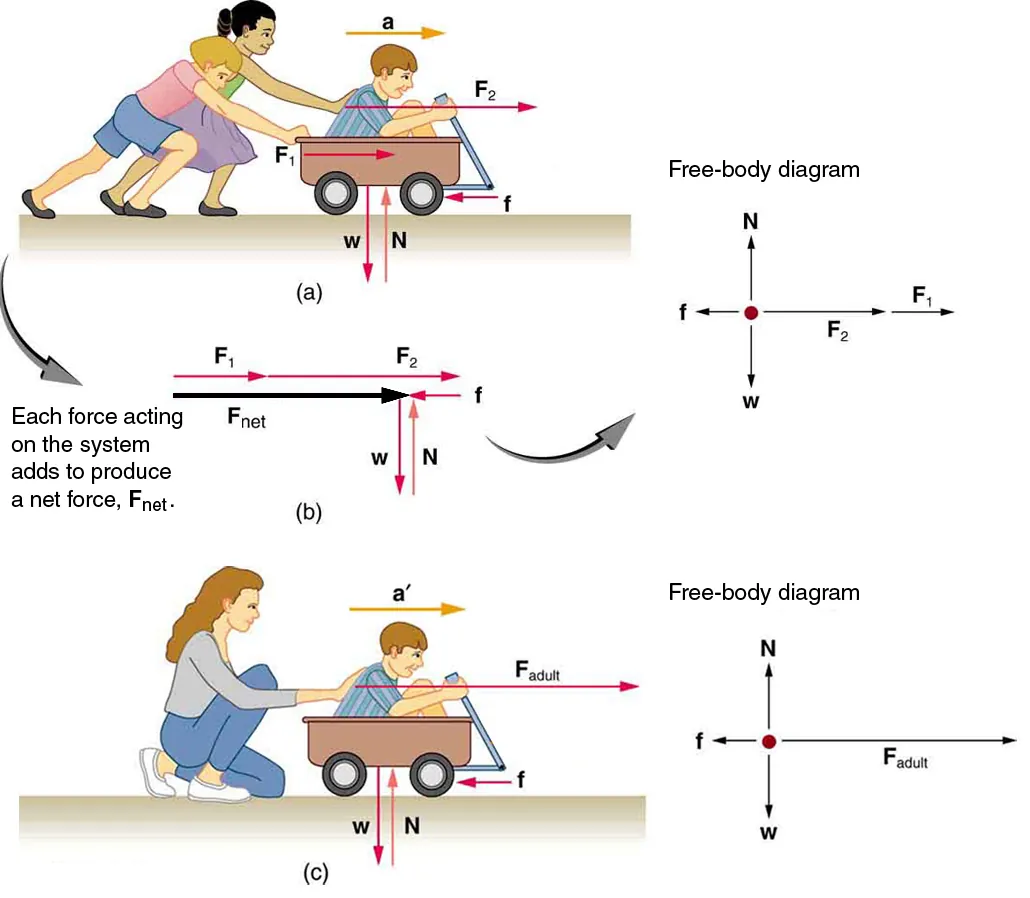
\includegraphics[width=0.75\linewidth]{freebody.png}
\end{center}

\subsection{Newton's First Law}

\theorem{Newton's first law}{A body at rest remains at rest, or, if in motion, remains in motion at a constant velocity unless acted on by a net external force.}

There must be a net external force to cause an object's velocity to change. Otherwise its current velocity is preserved. Only external forces will affect the object's velocity.

The property of a body to remain at the same velocity (or at rest) is called \textbf{inertia}. Newton's first law is also known as the law of inertia. Some objects have more inertia than others, which is how difficult/how much force is required to change its velocity.

The inertia of an object is determined by its \textbf{mass}. Weight is dependent on the object's location, but mass is constant everywhere.

\subsection{Newton's Second Law}

Acceleration is the change in an object's velocity. By Newton's first law, a net external force must cause acceleration. Acceleration also has the same direction (and is directly proportional) to the net external force that brought it about.

However, the acceleration is also affected by the mass of the object acted upon by the net external force. If the object is heavier (has more mass), it would require more force to accelerate it by the same amount than an object with lower mass.

\theorem{Newton's second law}{The acceleration of a system is directly proportional to and in the same direction as the net external force acting on the system, and inversely proportional to its mass.
\begin{equation*}
	\mathbf{a}=\frac{\mathbf{F}_{\text{net}}}{m}
	\iff
	\mathbf{F}_{\text{net}}=m \mathbf{a}
\end{equation*}
where $\mathbf{a}$ is acceleration, $\mathbf{F}_{\text{net}}$ is the net external force and $m$ is the mass of the system. Note that mass is a scalar, while force and acceleration are vectors.}

In $\mathbf{F}_{\text{net}}=m \mathbf{a}$, mass is measured in kilograms (kg) and acceleration is measured in meters per second squared (\si{\meter\per\second\squared}). The SI unit of force is the \textbf{newton} (N):
\begin{equation*}
	1\,\si{\newton}=1\,\si[inter-unit-product =\cdot]{\kilo\gram\meter\per\second\squared}
\end{equation*}

\subsection{Weight and Gravitational Force}

If air resistance is negligible, the net force acting on a falling object is \textbf{weight}. All objects fall with the same acceleration of $g$. The magnitude of weight is denoted $w$, and since near Earth the direction of weight is always downward, we can treat its magnitude alone.

$F_{\text{net}}$ is the net force acting upon a falling object. By definition, $w$ is the net force. By Newton's second law:
\begin{align*}
	F_{\text{net}}=
	w&=ma
	\intertext{We know acceleration is the gravitational constant $g$.}
	\implies \Aboxed{w&=mg}
\end{align*}

An object is in \textbf{free-fall} if the net external force on an object is exactly equivalent to its weight. The only force acting on the object is gravity.

The gravitational constant varies by location, so the weight of an object will vary by location. Since weight is a force, it is measured in newtons (N). Mass is always the same however.

\subsection{Newton's Third Law}
\theorem{Newton's third law}{Whenever one body exerts a force on a second body, the first body experiences a force that is equal in magnitude and opposite in direction to the force that it exerts.}

For example, when a swimmer's feet pushing against the wall of a swimming pool, the swimming pool wall will also exert a force of the same magnitude onto the swimmer, pushing them forward.

\subsection{Normal Force}

Weight acts on objects at all times, and therefore must be counteracted to keep an object stationary (and prevent it from falling further).

If an object is placed on a table, the force of gravity on the object will push down on the table. In turn, the table exerts a force of the same magnitude back onto the object due to Newton's third law.

\definition{The \textbf{normal force} is the force that surfaces exert to prevent solid objects from passing through each other.}

Normal force is often denoted with the symbol $\mathbf{N}$, which is \underline{\textbf{not}} the same as newtons (N). Normal force is not always the opposite weight, since the object could be on another surface that is itself moving or on an incline.

\subsection{Tension}

\definition{\textbf{Tension} is force along the length of a medium, especially a force carried along a flexible medium.}

Consider a mass attached to a rope. The tension in the rope must equal the force of gravity from the supported weight. (If the mass is stationary, then its acceleration is zero, then by Newton's second law $F_{\text{net}}=T-w=0\iff T=w=mg$ where $T$ is tension and $w$ is weight.)

\subsection{Friction}

\definition{\textbf{Friction} is a force that opposes relative motion between surfaces in contact.}

\definition{\textbf{Static friction} is friction between objects that are stationary relative to each other. \textbf{Kinetic friction} is friction between two surfaces that are moving relative to each other.}

Static friction is usually greater than kinetic friction.

Static friction is denoted $\mathbf{f}_{\text{s}}$. When there is no motion between surfaces, then:
\begin{equation*}
	\lVert \mathbf{f}_{\text{s}}\rVert =f_{\text{s}}\leq \mu_{\text{s}} N
\end{equation*}
where $N=\lVert \mathbf N \rVert $ is the magnitude of the normal force, and $\mu_{\text{s}}$ is the coefficient of static friction.

Static friction is a responsive force, its magnitude increases to be equal to whatever force is exerted onto the object. Once the applied force equals a maximum $f_{\text{s(max)}}$, the object will move, where $f_{\text{s(max)}}=\mu_{\text s}N$.

When the object is in motion, the magnitude of kinetic friction, denoted $\mathbf{f}_{\text{k}}$, is given by:
\begin{equation*}
	\lVert \mathbf{f}_{\text{k}}\rVert =f_{\text{k}}=\mu_{\text{k}} N
\end{equation*}
where $\mu_{\text{k}}$ is the coefficient of kinetic friction. If this is true, then the system is one where friction behaves simply.

The magnitude of kinetic friction is the same regardless of the force applied to the object. In order to move an object with an acceleration $a$, the magnitude of the force applied has to be:
\begin{align*}
	F
	&=\lVert \mathbf{f}_{\text{k}} \rVert +ma
	=\mu_{\text{k}}N+ma \\
	\intertext{If the surface the object is on is flat, i.e. There is no incline, then $N=w=mg$.}
	&=\mu_{\text{k}}mg+ma
\end{align*}

$N$ may not always be only weight. $N$ measures the force pushing the object into the surface, so if there is another force $F$ pushing it down or lifting it up, we would calculate friction $F=\mu (N\pm F)$.

\section{Energy}

\definition{\textbf{Energy} can be loosely defined as the ability to do work.}

\subsection{Work}

\definition{The \textbf{work} done on a system by a constant force is the product of the component of the force in the direction of motion times the distance through which the force acts. Work is denoted $W$:
\begin{equation*}
    W=\lVert \mathbf{F} \rVert \lVert \mathbf{d} \rVert \cos \theta
\end{equation*}
where $\mathbf{F}$ is the force vector, $\mathbf{d}$ is the displacement through which the force acts, and $\theta$ is the angle between the force vector and the displacement vector.
}

For one way motion in one direction, the equation can be written as:
\begin{equation*}
    W=Fd\cos\theta
\end{equation*}

There must be a displacement for work to be done, and the force applied must also have a component in the direction of the motion/displacement. Work can also be negative, which happens when $\cos\theta<0$.

Work is force (measured in newtons) multiplied by a displacement (measured in meters) and a scalar ($\cos\theta$). Thus, work is measured in newton-meters. A newton-meter is called a \textbf{Joule} (J).
\begin{equation*}
	1\,\si{\joule}
	=1\,\si[inter-unit-product=\cdot]{\newton\meter}
	=1\,\si[inter-unit-product=\cdot]{\kilo\gram\meter\squared\per\second\squared}
\end{equation*}

\definition{\textbf{Net work} is the sum of work done on an object. It can be written as:
\begin{equation*}
	W_{\text{net}}=\lVert \mathbf{F}_{\text{net}} \rVert \lVert \mathbf{d} \rVert \cos \theta
\end{equation*}
}

More generally, if force varies, then net work is the integral of the component of force in the direction of the displacement with respect to distance:
\begin{equation*}
    W=\int_{0}^{d}\mathbf{F}\cos\theta\,\mathrm{d}x
\end{equation*}

\subsection{Kinetic Energy and the Work-Energy Theorem}

Consider a net force pushing an object in one direction. The direction of the force is the same as direction of displacement, hence $\theta=0$ and $\cos\theta=1$.
\begin{align*}
	W_{\text{net}}
	&=F_{\text{net}}d\cos\theta=F_{\text{net}}d
	\intertext{Substituting $F_{\text{net}}=ma$ by Newton's second law:}
	W_{\text{net}}
	&=mad
	\intertext{where $m$ is mass, $a$ is acceleration and $d$ is displacement. We can find $a$ in terms of $v_0$ and $v$, the initial and final velocity. From the kinematic equation $v^2=v_0^2+2ad \implies a=(v^2-v_0^2)/(2d)$.}
	W_{\text{net}}
	&=m \left( \frac{v^2-v_0^2}{2d} \right)d \\
	\Aboxed{W_{\text{net}}
	&=\frac12mv^2-\frac12mv_0^2}
\end{align*}

\definition{\textbf{Kinetic energy} is the form of energy an object possesses due to motion. The translational kinetic energy object $\text{KE}$ is given by:
\begin{equation*}
    \text{KE}=\frac12mv^2
\end{equation*}
where $m$ is the object's mass and $v$ is the magnitude of its velocity.}

Thus, in the above equation for $W_{\text{net}}$, the net work on an object equals the change in kinetic energy. ($mv^2/2$ is the final kinetic energy, and $mv_0^2/2$ is the initial kinetic energy.) This is the \textbf{work-energy theorem}.

\theorem{Work-energy theorem}{The net work on a system equals the change in kinetic energy $\Delta \text{KE}$:
\begin{equation*}
	W_{\text{net}}
	=\Delta \text{KE}
	=\frac12mv^2-\frac12mv_0^2
\end{equation*}
where $m$ is the mass of the object, $v_0$ is the magnitude of the object's initial velocity and $v$ is the magnitude of the object's final velocity.}

\subsection{Gravitational Potential Energy}

The force needed to lift an object is equal to its weight, that is $F=mg$. The work done on the mass to lift it to height $h$ is $W=Fd\cos\theta=mgh$, since $\theta=0$.

\definition{\textbf{Gravitational potential energy} is a form of energy stored in an object due to its position in a gravitational force. An object's gravitational potential energy $\text{PE}_\text{g}$ equals the work done on an object to raise it a certain height $h$ above a reference point where gravitational potential energy is zero:
\begin{equation*}
	\text{PE}_{\text{g}}=mgh
\end{equation*}
where $g$ is the gravitational constant of the gravitational field and $m$ is the mass of the object.}

The reference level where $\text{PE}_\text{g}=0$ is usually set to the surface of the Earth. This point can be chosen arbitrarily however, since difference in gravitational potential energy is more important than the value of $\text{PE}_\text{g}$ itself.

The change in gravitational potential energy $\Delta \text{PE}_\text{g}$ can be calculated by the same equation:
\begin{equation*}
    \Delta \text{PE}_\text{g}=mg\Delta h
\end{equation*}
where $\Delta h$ is the change in height.

Since energy is conserved, the kinetic energy associated with the change in height $\Delta \text{KE}=-\Delta \text{PE}_\text{g}$.

\subsection{Potential Energy and Conservative Forces}

\definition{\textbf{Potential energy} ($\text{PE}$) is the energy a system has due to position, shape, or configuration. It is stored energy that is completely recoverable.}

\definition{A \textbf{conservative force} is one for which work done by or against it depends only on the starting and ending points of a motion and not on the path taken.}

A potential energy can be defined for any conservative force, because the work done by/against a conservative force is affected by configuration and not by the path along which the force acts.

\subsection{Potential Energy of a Spring}

Hooke's Law states that the force created by a spring, extended or compressed by distance $x$, is given by (where $k$ is the spring's force constant):
\begin{equation*}
    F=kx
\end{equation*}
To calculate the work done by extending or compressing the spring, we apply the force along the distance $x$. This also equals the \textbf{potential energy of the spring}:
\begin{equation*}
	\text{PE}_{\text{s}}
	=W_\text{s}
	=\int_{0}^{x}ks\,\mathrm{d}s
	=\left[\frac12 ks^2\right]_{0}^{x}
	=\frac12 kx^2
\end{equation*}

\subsection{Conservation of Mechanical Energy}

\definition{\textbf{Mechanical energy} ($\text{ME}$) is the total kinetic energy of a system plus its total potential energy.
\begin{equation*}
	\text{ME}=\text{KE}+\text{PE}
\end{equation*}}
If only conservative forces act upon a system, then net work equals work from conservative forces. By the work-energy theorem:
\begin{equation*}
	\Delta \text{KE}=W_{\text{net}}=W_{\text{c}}
\end{equation*}
Work done by a conservative force comes at a loss of potential energy (for example, $\text{PE}_\text{g}$ is lost in a falling object). Since energy is conserved:
\begin{equation*}
	\Delta \text{KE}+\Delta \text{PE}=\Delta \text{ME}=0
	\iff \Delta \text{KE}=-\Delta \text{PE}
	\iff W_\text{net}=W_\text{c}=-\Delta \text{PE}
\end{equation*}
In systems with only conservative forces, energy only changes form between kinetic energy and various forms of potential energy. The total mechanical energy in the system remains constant.
\begin{align*}
	\text{PE}+\text{KE}&=\text{ME} \\
	\text{PE}_\text{i}+\text{KE}_\text{i}&=\text{PE}_\text{f}+\text{KE}_\text{f}
\end{align*}

\subsection{Nonconservative Forces}

\definition{A \textbf{nonconservative force} is a force for which its work depends on the path taken.}

Unlike conservative forces, nonconservative forces add or remove mechanical energy from a system.

For example, work done by friction depends on the length of the path/distance traveled between the starting and ending point. Friction removes energy from the system by converting it to thermal energy, which is lost/cannot be recovered.

Mechanical energy (ME) may not be conserved if nonconservative forces act upon the system. (For example, a rock that is dropped loses both its KE and $\text{PE}_\text{g}$ from nonconservative forces when it hits the ground.)

Let $W_{\text{c}},W_{\text{nc}}$ denote work from conservative and nonconservative forces, respectively. By the work-energy theorem:
\begin{align*}
	W_{\text{net}}
	&=\Delta \text{KE}
	=W_{\text{c}}+W_{\text{nc}} \\
	\intertext{From previously, $W_\text{c}=-\Delta \text{PE}$.}
	\Delta \text{KE}
	&=-\Delta \text{PE}+W_\text{nc} \\
	W_\text{nc}
	&=\Delta \text{KE}+\Delta \text{PE} \\
	W_\text{nc}
	&=\text{KE}_\text{f}-\text{KE}_\text{i}+\text{PE}_\text{f}-\text{PE}_\text{i} \\
	\text{KE}_\text{i}+\text{PE}_\text{i}+W_\text{nc}
	&=\text{KE}_\text{f}+\text{PE}_\text{f}
\end{align*}

If $W_\text{nc}>0$, then nonconservative forces add energy to the system, and mechanical energy is increased. If $W_\text{nc}<0$, then mechanical energy is decreased. If $W_\text{nc}=0$, then mechanical energy is conserved. (If only conservative forces act on the system, mechanical energy is conserved because $W_\text{nc}=0$.)

\subsection{Conservation of Energy}

There are forms of energy other than mechanical energy (kinetic and potential energy). We can group these into other energy ($\text{OE}$). We can write the conservation of energy equation as:
\begin{equation*}
	\text{KE}_\text{i}+\text{PE}_\text{i}+\text{OE}_\text{i}+W_\text{nc}=\text{KE}_\text{f}+\text{PE}_\text{f}+\text{OE}_\text{f}
\end{equation*}
Kinetic energy is KE, work done by conservative forces is PE, work done by nonconservative forces is $W_\text{nc}$ and work from other forms of energy is OE. Subscripts i and f indicate initial and final.

\theorem{Conservation of energy}{Total energy is constant in any process. It may change in form or be transferred from one system to another, but the total remains the same.

If KE is kinetic energy, PE is potential energy derived from conservative forces, OE is other forms of energy and $W_\text{nc}$ is work done by nonconservative forces, then:
\begin{align*}
	\Delta \text{KE}+\Delta \text{PE}&=W_{\text{nc}} \\
	\text{KE}_\text{i}+\text{PE}_\text{i}+\text{OE}_\text{i}+W_\text{nc}
	&=\text{KE}_\text{f}+\text{PE}_\text{f}+\text{OE}_\text{f}
\end{align*}
If only conservative forces act upon a system, then $W_{\text{nc}}=0$. The total mechanical energy ($\text{ME}=\text{KE}+\text{ME}$) of the system is constant:
\begin{align*}
	\text{KE}_\text{i}+\text{PE}_\text{i}+\text{OE}_\text{i}&=\text{KE}_\text{f}+\text{PE}_\text{f}+\text{OE}_\text{f}
	\intertext{If other energy does not change, then $\text{OE}_\text{i}=\text{OE}_\text{f}$. This is known as \textbf{conservation of mechanical energy}:}
	\text{KE}_\text{i}+\text{PE}_\text{i}&=\text{KE}_\text{f}+\text{PE}_\text{f}
\end{align*}}

Other forms of energy include: electrical energy, chemical energy, nuclear energy and thermal energy.

\subsection{Efficiency}

The output of useful energy will be less than the energy input, since some of the energy will be wasted or lost (for example, friction converts some energy to sound and thermal energy). Efficiency (Eff) measures how much input energy is converted to useful energy:
\begin{equation*}
	\text{Eff}=\frac{\text{useful energy or work output}}{\text{total energy input}}=\frac{W_\text{out}}{E_\text{in}}
\end{equation*}

\subsection{Power}

\definition{\textbf{Power} ($P$) is the rate at which work is done: If $W$ is work and $t$ is time:
\begin{equation*}
    P=\frac{W}{t}
\end{equation*}}

The SI unit for work is the \textbf{watt} (W), which is equivalent to joules (unit of work) per second (unit of time).
\begin{equation*}
	1\,\si{\watt}
	=1\,\si{\joule\per\second}
	=1\,\si{(\newton\cdot\meter)\per\second}
\end{equation*}

\section{Momentum}

\subsection{Linear Momentum}

\definition{The \textbf{linear momentum} ($\mathbf p$) of a system is its the product of its mass and its velocity. Linear momentum is a vector.
\begin{equation*}
	\mathbf{p}=m \mathbf{v}
\end{equation*}
where scalar $m$ is mass and vector $\mathbf{v}$ is velocity.}
The SI unit for momentum is \si{\kilogram\cdot\meter\per\second}. Momentum $\mathbf{p}$ has the same direction as velocity $\mathbf{v}$.

\theorem{Newton's second law in terms of momentum}{Net external force equals the change in momentum of a system divided by the time over which it changes.
\begin{equation*}
	\mathbf{F}_\text{net}=\frac{\Delta \mathbf{p}}{\Delta t}
\end{equation*}
}

$\mathbf{F}_\text{net}=m \mathbf{a}$ is a special case when mass $m$ is constant. If mass $m$ is constant, then $\Delta \mathbf{p}=\Delta (m \mathbf{v})$ becomes $m \Delta \mathbf{v}$:
\begin{align*}
	\mathbf{F}_\text{net}&=\frac{m\Delta \mathbf{v}}{\Delta t}
	\intertext{Acceleration $\mathbf{a}$ is the change of velocity over time: $\mathbf{a}=\Delta \mathbf{v}/\Delta t$.}
	\mathbf{F}_\text{net}&=m \mathbf{a}
\end{align*}

\subsection{Impulse}

The ability of a force to change an object's momentum depends on the magnitude of the force and the time over which it acts. From Newton's second law:
\begin{equation*}
	\mathbf{F}_\text{net}=\frac{\Delta \mathbf{p}}{\Delta t}
	\implies
	\Delta \mathbf{p}=\mathbf{F}_\text{net}\Delta t
\end{equation*}

\definition{Change in momentum is the total net external force applied over time. If the net external force $\mathbf{F}_\text{net}$ is constant:
\begin{equation*}
	\Delta \mathbf{p}=\mathbf{F}_\text{net}\Delta t
\end{equation*}
If it varies, then the change in momentum between time $t=a$ and time $t=b$ is given by:
\begin{equation*}
	\Delta \mathbf{p}=\int_{a}^{b}\mathbf{F}_\text{net}\,\mathrm{d}t
\end{equation*}
These equal each other if $\mathbf{F}_\text{net}$ is constant. The quantity $\int_{a}^{b}\mathbf{F}_\text{net}\,\mathrm{d}t \stackrel{?}{=} \mathbf{F}_\text{net}\Delta t$ is the \textbf{impulse}.}

\subsection{Conservation of momentum}

\definition{An \textbf{isolated system} is one where the net external force $\mathbf{F}_\text{net}=0$.}

\theorem{Conservation of momentum}{The total momentum $\mathbf{p}_\text{tot}$ (the sum of the momentum of each object in the system) of any isolated system is conserved. $\mathbf{p}_\text{tot}'$ is the total momentum of the system some time later.
\begin{align*}
	\mathbf{p}_\text{tot}&=\text{constant} \\
	\mathbf{p}_\text{tot}&=\mathbf{p}_\text{tot}'
\end{align*}}

If the system is isolated and $\mathbf{F}_\text{net}=0$, then from Newton's second law, there is no change in momentum:
\begin{equation*}
	\mathbf{F}_\text{net}=\frac{\Delta \mathbf{p}_\text{tot}}{\Delta t}
	\implies \frac{\Delta \mathbf{p}_\text{tot}}{\Delta t}=0
	\implies \Delta \mathbf{p}_\text{tot}=0
\end{equation*}


\section{Collisions}

\subsection{1D Elastic Collisions}

\definition{The \textbf{internal kinetic energy} of a system is the sum of the kinetic energies of all objects in the system. An \textbf{elastic collision} is one that conserves internal kinetic energy.}

Consider two objects with masses $m_1,m_2$ and traveling at velocity $v_1,v_2$. They will have kinetic energy $\text{KE}_1,\text{KE}_2$:
\begin{equation*}
	\text{KE}_1=\frac12 m_1(v_1)^2
	\qquad
	\text{KE}_2=\frac12 m_2(v_2)^2
\end{equation*}
$v_1',v_2'$ are the objects' velocities after the collision. They will have kinetic energy $\text{KE}_1',\text{KE}_2'$:
\begin{equation*}
	\text{KE}_1'=\frac12 m_1(v_1')^2
	\qquad
	\text{KE}_2'=\frac12 m_2(v_2')^2
\end{equation*}
Since the collision is elastic, the internal kinetic energies are conserved:
\begin{align*}
	\text{KE}_1+\text{KE}_2&=\text{KE}_1'+\text{KE}_2' \\
	\Aboxed{\frac12 m_1(v_1)^2+\frac12 m_2(v_2)^2&=\frac12 m_1(v_1')^2+\frac12 m_2(v_2')^2}
\end{align*}
If there is no net external force $\mathbf{F}_ \text{net}t=0$, then momentum is also conserved. Total momentum $\mathbf{p}_\text{tot}=\mathbf{p}_1+\mathbf{p}_2$, where $\mathbf{p}_1,\mathbf{p}_2$ are the momentum of each object before the collision.
\begin{align*}
    \mathbf{p}_ \text{tot}&=\mathbf{p}_ \text{tot}' \\
	\mathbf{p}_1+\mathbf{p}_2&=\mathbf{p}_1'+\mathbf{p}_2'
	\intertext{By definition of momentum, $\mathbf{p}_x=m_x \mathbf{v}_x$. Supposing mass does not change from the collision.}
	\Aboxed{m_1\mathbf{v}_1+m_2\mathbf{v}_2&=m_1\mathbf{v}_1'+m_2\mathbf{v}_2'}
\end{align*}

\subsection{1D Inelastic Collisions}

\definition{An \textbf{inelastic collision} is one where internal kinetic energy changes and is not conserved.}

In an inelastic collision, forces between may add or remove internal kinetic energy (changing the total energy of objects in the system), such as dissipating some kinetic energy into heat.

\definition{A \textbf{perfect inelastic collision} is one where the objects stick together after a collision (the objects' relative velocities to each other is $0$).}

A perfect inelastic collision reduces the internal kinetic energy of a system by as much as possible while still conserving momentum.

\subsection{2D Collisions of Point Masses Where One is Stationary}

\definition{A \textbf{point mass} is a hypothetical object with mass but cannot rotate or spin.}

We consider point masses only for now because we do not want to consider rotation. Similar to kinematics, we can consider the $x$ and $y$ components of each object and the collision separately.

Suppose there are two point masses. The second object is stationary (with $v_2=0$). We define the coordinate system such that the first object's momentum in the $y$ direction $p_y=0$ and $p_x$ equals its momentum. Let $m_1,m_2$ be the masses of the two point masses.

Define angles $\theta_1$ and $\theta_2$ be the angle between object 1's initial velocity vector $v_1$ and $v_1'$ and $v_2'$, where $v_1',v_2'$ are the velocities of the two point masses after the collision.

Also suppose that $\mathbf{F}_ \text{net}=0$ so that momentum is conserved.

\begin{center}
	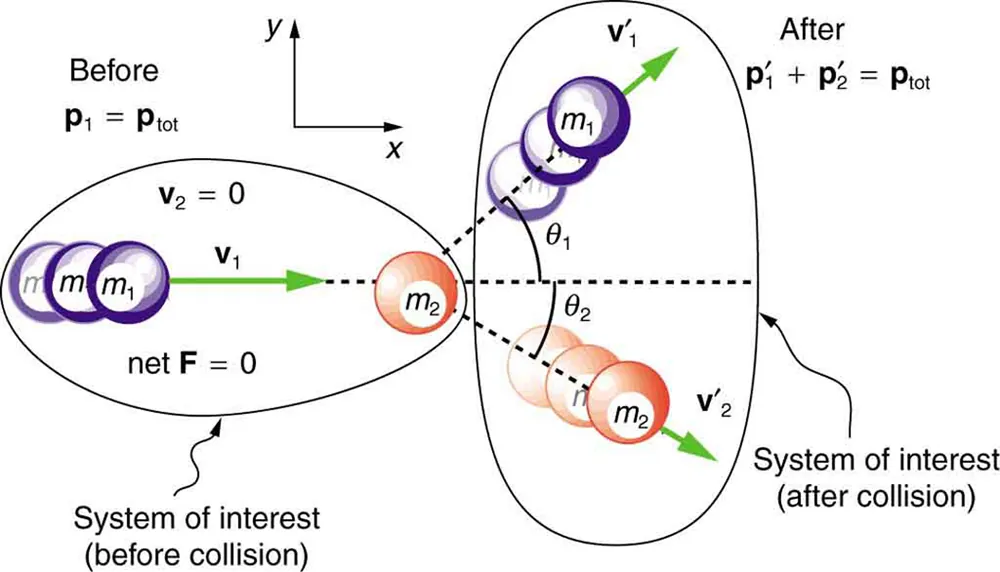
\includegraphics[width=0.8\linewidth]{2dcollision.png}
\end{center}

By conservation of momentum:
\begin{align*}
	\mathbf{p}_ \text{tot}&=\mathbf{p}_ \text{tot}'
	\intertext{In the $x$ direction (defined such that object 1 is only moving in this direction):}
	p_{1x}+p_{2x}&=p_{1x}'+p_{2x}' \\
	m_1v_{1x}+m_2v_{2x}&=m_1v_{1x}'+m_2v_{2x}'
	\intertext{where $p_{1x}$ is object 1's momentum in the $x$ direction, $v_{1x}$ is object 1's velocity in the $x$ direction, etc. Since object 2 is stationary, $v_{2x}=0$.}
	m_1v_{1x}&=m_1v_{1x}'+m_2v_{2x}'
	\intertext{The coordinate system is defined such that all of object 1's initial velocity is in the $x$ direction, so $v_1=v_{1x}$. We do not know this for $v_{1x}'$ and $v_{2x}'$, as those are after the collision. These can be determined by trigonometry.}
	\Aboxed{m_1v_1&=m_1v_1'\cos\theta_1+m_2v_2'\cos\theta_2}
\end{align*}
This is the conservation of momentum in the $x$ direction/along the $x$-axis. Similarly in the $y$ direction (noting that the coordinate system is defined so that $v_{1y}=0$):
\begin{align*}
	p_{1y}+p_{2y}&=p_{1y}'+p_{2y}' \\
	0&=m_1v_{1y}'+m_2v_{2y}' \\
	\Aboxed{0&=m_1v_1'\sin\theta_1+m_2v_2'\sin\theta_2}
\end{align*}

\subsubsection{Elastic collisions between two objects of equal mass}

We find the cases when the collision is elastic, i.e. the internal kinetic energy is conserved. As before, suppose object 2 starts at rest. As before, the coordinate system is defined such that $p_{1x}=p_1$ and $p_{1y}=0$. The two objects are of equal mass $m$. From before (conservation of momentum):
\begin{align}
	m_1v_1&=m_1v_1'\cos\theta_1+m_2v_2'\cos\theta_2 \notag \\
	0&=m_1v_1'\sin\theta_1+m_2v_2'\sin\theta_2 \notag
	\intertext{The masses are equal: $m_1=m_2=m$. Since $m\neq0$, divide both sides by $m$.}
	v_1&=v_1'\cos\theta_1+v_2'\cos\theta_2 \\
	0&=v_1'\sin\theta_1+v_2'\sin\theta_2
\end{align}
We calculate the internal kinetic energy before the collision is (call this $\text{KE}$, which equals the kinetic energy of object 1), and do some algebraic manipulations to write it into a form that we can determine when $\text{KE}$ equals the internal kinetic energy after the collision $\text{KE}'$.
\begin{align*}
	\text{KE}
	&=\frac12 mv_1^2 \\
	&=\frac12m\left(v_1'\cos\theta_1+v_2'\cos\theta_2\right)^2 \\
	&=\frac12m\left((v_1')^2\cos^2\theta_1+2(v_1')(v_2')\cos\theta_1\cos\theta_2+(v_2')^2\cos^2\theta_2\right) \\
	&=\frac12m(v_1')^2\cos^2\theta_1+\frac12m(v_2')^2\cos^2\theta_2+m(v_1')(v_2')\cos\theta_1\cos\theta_2 \\
	&=\frac12m(v_1')^2 \left( 1-\sin^2\theta_1 \right)+\frac12m(v_2')^2 \left( 1-\sin^2\theta_2 \right)+m(v_1')(v_2')\cos\theta_1\cos\theta_2 \\
	&=\frac12 m(v_1')^2+\frac12m(v_2')^2-\frac12m(v_1')^2\sin^2\theta_1-\frac12m(v_2')^2\sin^2\theta_2+m(v_1')(v_2')\cos\theta_1\cos\theta_2 \\
	&=\frac12 m(v_1')^2+\frac12m(v_2')^2+m\left((v_1')(v_2')\cos\theta_1\cos\theta_2-\frac12(v_1')^2\sin^2\theta_1-\frac12(v_2')^2\sin^2\theta_2\right) \\
	\intertext{We consider the last two terms, $-(v_1')^2\sin^2\theta_1/2-(v_2')^2\sin^2\theta_2/2$ separately. We use equation (2) from earlier.
	\begin{mdframed}
		$\begin{aligned}[t]
			&-\frac12(v_1')^2\sin^2\theta_1-\frac12(v_2')^2\sin^2\theta_2
			=(-1/2)\left((v_1')^2\sin^2\theta_1+(v_2')^2\sin^2\theta_2\right) \\
			={}&(-1/2)\left((v_1')^2\sin^2\theta_1+2(v_1')(v_2')\sin\theta_1\sin\theta_2+(v_2')^2\sin^2\theta_2-2(v_1')(v_2')\sin\theta_1\sin\theta_2\right) \\
			={}&(-1/2)\left(\left( v_1'\sin\theta_1+v_2'\sin\theta_2 \right)^2-2(v_1')(v_2')\sin\theta_1\sin\theta_2\right)
			=(-1/2)\left(-2(v_1')(v_2')\sin\theta_1\sin\theta_2\right) \\
			={}&(v_1')(v_2')\sin\theta_1\sin\theta_2
		\end{aligned}$
	\end{mdframed}}
	&=\frac12 m(v_1')^2+\frac12m(v_2')^2+m\left((v_1')(v_2')\cos\theta_1\cos\theta_2+(v_1')(v_2')\sin\theta_1\sin\theta_2\right) \\
	&=\frac12 m(v_1')^2+\frac12m(v_2')^2+m(v_1')(v_2')\left(\cos\theta_1\cos\theta_2+\sin\theta_1\sin\theta_2\right) \\
	\intertext{By cosine subtraction identity $\cos(a-b)=\cos a\cos b+\sin a\sin b$:}
	\Aboxed{\text{KE}&=\frac12 m(v_1')^2+\frac12m(v_2')^2+m(v_1')(v_2')\cos(\theta_1-\theta_2)}
	\intertext{Next, we calculate the internal kinetic energy of the two objects after the collision $\text{KE}'$:}
	\Aboxed{\text{KE}'&=\frac12 m(v_1')^2+\frac12m(v_2')^2}
\end{align*}

We aim to find when the collision is elastic, i.e. the internal kinetic energy is not changed by the collision: $\text{KE}=\text{KE}'$. This is exactly when:
\begin{equation*}
    m(v_1')(v_2')\cos(\theta_1-\theta_2)=0
\end{equation*}
The cases where this is true are:
\begin{itemize}
    \item $v_1'=0$: object 1 transfers all its momentum to object 2, causing object 1 to come to a stop. This occurs when there is a head-on collision between two balls of equal mass, as we have specified.
	\item $v_2'=0$: object 2 is still stationary, meaning no momentum has been transferred and there is actually no collision at all.
	\item $\cos(\theta_1-\theta_2)=0 \impliedby \theta_1-\theta_2=\pi/2=90^\circ$: the angle of separation between the two objects after the collision is $90^\circ$.
\end{itemize}

\section{Circular Motion}

\definition{When an object rotates around an axis: $\Delta \theta$ is used for \textbf{rotation angle}, $\Delta s$ for \textbf{arc length} and $r$ for \textbf{radius of curvature}.}

Rotation angle $\Delta \theta$ is measured in radians (\si{rad}).

\definition{\textbf{Angular velocity} is the rate of change of an angle, denoted $\omega$ (lowercase Greek letter omega).
\begin{equation*}
    \omega=\frac{\Delta \theta}{\Delta t}
\end{equation*}
where an angular rotation $\Delta \theta$ takes place in time $\Delta t$.}

Angular velocity is measured in radians per second (\si{\radian\per\second}).

The angular velocity is related to the same object's linear velocity. The linear velocity is the rate of change of arc length $\Delta s$ with respect to time:
\begin{equation*}
    v=\frac{\Delta s}{\Delta t}
\end{equation*}
But also, arc length can be given in terms of radius of curvature $r$ and the rotation angle $\Delta \theta$:
\begin{equation*}
    \Delta s=r\Delta\theta
\end{equation*}
So we can write the linear velocity in terms of the angular velocity, and vice versa:
\begin{equation*}
    v=\frac{r\Delta \theta}{\Delta t}=r \left( \frac{\Delta\theta}{\Delta t} \right)=r\omega
	\iff 
	\omega=\frac{v}{r}
\end{equation*}

\theorem*{If an object is rotating around some axis with radius of curvature $r$, then the relationship between linear velocity and angular velocity is:
\begin{equation*}
	v=r\omega \qquad \omega=\frac{v}{r}
\end{equation*}}
Thus, the linear velocity $v$ is proportional to the distance to the center of rotation. Both $v$ and $\omega$ have directions (since they are velocity, not speed), the directions are clockwise and counterclockwise.

\subsection{Centripetal Acceleration}

\definition{An object is in \textbf{Uniform circular motion} if travels at a constant speed on a circular path. \textbf{Centripetal acceleration} $\mathbf{a}_ \text{c}$ is the acceleration of an object in uniform circular motion.}

Centripetal acceleration is a vector. By handwavery, at any time, an object's centripetal acceleration/the vector $\mathbf{a}_ \text{c}$ points to the center of curvature. The magnitude of centripetal acceleration is given by:
\begin{equation*}
    \lVert \mathbf{a}_ \text{c} \rVert 
	=a_ \text{c}
	=\frac{v^2}{r}
	=r \omega^2
\end{equation*}
where $v$ is the magnitude of the object's linear velocity (given by $v=\Delta s/\Delta t$), $r$ is the radius of curvature and $\omega$ is the object's angular velocity (given by $\omega=\Delta \theta/\Delta \theta=v/r$).

Centripetal acceleration/centripetal force affects the object's direction of motion, but not the magnitude of velocity/speed.

\subsection{Centripetal Force}

\definition{\textbf{Centripetal force} is a net force causing uniform circular motion.}

When an object is in uniform circular motion, the same object's direction of centripetal force is towards the center of curvature, which is the same as the direction of centripetal acceleration $\mathbf{a}_ \text{c}$.

Centripetal force is denoted $\mathbf{F}_\text{c}$. The magnitude of centripetal force can be found from Newton's second law:
\begin{align*}
	\lVert \mathbf{F}_\text{c} \rVert =F_\text{c}
	&=ma_\text{c}
	\intertext{We know from before that the magnitude of centripetal acceleration $a_\text{c}=v^2/r=r\omega^2$.}
	\Aboxed{F_\text{c}
	&=\frac{mv^2}{r}
	=mr\omega^2}
	\intertext{Rearranging and solving for radius of curvature $r$ gives:}
	r
	&=\frac{mv^2}{F_\text{c}}
\end{align*}
Since the radius of curvature is inversely proportional to centripetal force, a higher centripetal force results in a smaller radius of curvature, and a tighter curve/motion.

\subsubsection{Banked curves}

This is an example application of centripetal force. In the free body diagram below, the car is traveling on a banked road. We want to calculate the angle $\theta$ such that the car can drive the curve without using tire friction. This occurs when the net external force is exactly the centripetal force needed to put the car in uniform circular motion.
\begin{center}
	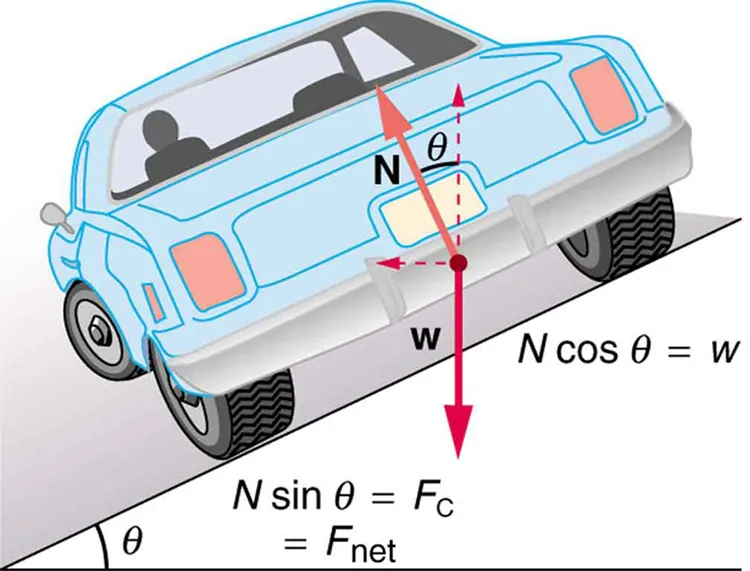
\includegraphics[width=0.6\linewidth]{centripetalcar.png}
\end{center}
$\mathbf{N}$ is normal force, $\mathbf{w}$ is weight and $\mathbf{F}_\text{c}$ is centripetal force. Non-bold denotes magnitude.

First, the car stays on the ground, meaning the vertical component of the normal force (the normal force has a horizontal component, since the ground is inclined) must equal weight/force of gravity.
\begin{align*}
	N\cos\theta&=w=mg 
	\intertext{There is also a component of normal force pushing the car left, an amount which equals the centripetal force.}
	N\sin\theta&=F_\text{c}=\frac{mv^2}{r}
\end{align*}
Dividing these equations, we have:
\begin{equation*}
	\frac{N\sin\theta}{N\cos\theta}=\frac{\cancel{m}v^2}{\cancel{m}gr}
	\implies \tan\theta=\frac{v^2}{gr}
	\implies \boxed{\theta=\arctan\left(\frac{v^2}{gr}\right)}
\end{equation*}
This is the angle the road must be banked in order for the car to enter circular motion of radius $r$ at velocity $v$ without using any other external forces like tire friction.

\section{Rotational Kinematics}

\subsection{Torque}

\definition{\textbf{Torque} $\boldsymbol{\tau}$ is the rotational equivalent of force. Torque is a vector quantity. Torque measures how effectively a force is able to change the angular velocity of an object. The magnitude of torque $\tau$ is defined as:
\begin{equation*}
	\tau=rF\sin\theta
\end{equation*}
where $F$ is the magnitude of the force applied, $r$ is the distance between the pivot point and where the force is applied, $\theta$ is the angle between the force vector and the vector between the pivot point and where the force is applied.}
\begin{center}
	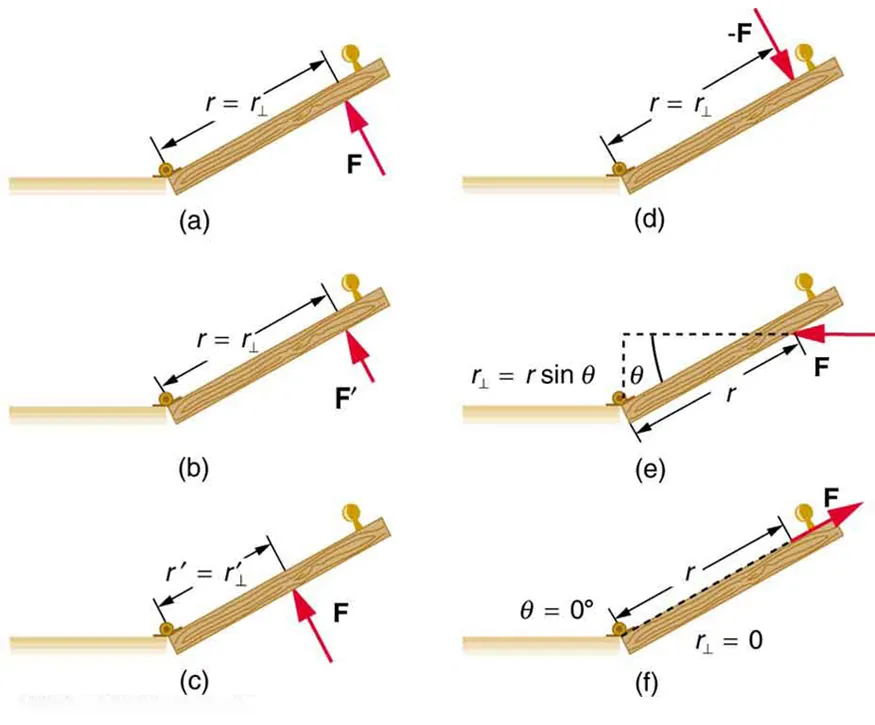
\includegraphics[width=0.8\linewidth]{torque.png}
\end{center}
\definition{The \textbf{perpendicular lever arm} $r_\perp$ is the shortest distance from the pivot point to the line created by extending the force vector $\mathbf{F}$. By trigonometry, the formula for $r_\perp$ is:
\begin{equation*}
    r_\perp=r\sin\theta
\end{equation*}
where $r,\theta$ are the same as defined previously. Torque can also be written as:
\begin{equation*}
    \tau=r_\perp F
\end{equation*}}
Torque is measured in newton-meters (\si{\newton\cdot\meter}). In the formula for magnitude of torque $\tau=rF\sin\theta$, radius $r$ is measured in meters, magnitude of force $F$ is measured in newtons, and $\sin\theta$ is a scalar.

Torque is proportional to the perpendicular lever arm. If the magnitude of force remains the same, torque is highest when $\theta=90^\circ\implies \sin\theta=1$, which is also the maximum length of the perpendicular lever arm.

It is common to define counterclockwise torque as positive and clockwise as negative (same as unit circle).

\theorem{Torque and angular acceleration}{The relationship between torque and angular acceleration is:
\begin{equation*}
    \tau=I\alpha
\end{equation*}
where $\alpha$ is angular acceleration and $I$ is the \textbf{moment of inertia}. Usually (but not always), the moment of inertia $I=mr^2/2$, where $m$ is the object's mass and $r$ is the radius/distance from where the force is applied to the pivot point.}

\theorem{Rotational kinetic energy}{The kinetic energy of an object moving at angular velocity $\omega$ is:
\begin{equation*}
	\text{KE}_\text{rotational}=\frac12I\omega^2
\end{equation*}
where $I$ is the moment of inertia. An object's total kinetic energy is the sum of rotational kinetic energy and linear kinetic energy:
\begin{equation*}
	\text{KE}=\frac12mv^2+\frac12I\omega^2=\frac12mv^2+\frac12 \frac{v^2}{r^2}I
\end{equation*}}

\subsection{Angular Momentum}

\theorem{Angular momentum}{The equation for angular momentum $L$ and change in angular momentum $\Delta L$ are:
\begin{equation*}
	L=I\omega \qquad
	\Delta L=\tau_\text{avg}\Delta t
\end{equation*}
where $I$ is the moment of inertia, $\omega$ is angular velocity, $\tau_\text{avg}$ is average torque, $\Delta t$ is elapsed time.}

\subsection{Equilibrium}

\definition{\textbf{Equilibrium} is a state when the forces acting on an object that is stationary (not moving) or moving at a constant velocity are balanced.}

It is necessary for the net external force $\mathbf{F}_\text{net}=0$. However, it is not sufficient. In this case, $\mathbf{F}_\text{net}=0$, but the object's rotation will accelerate, meaning it is not in equilibrium (forces are not balanced).
\begin{center}
	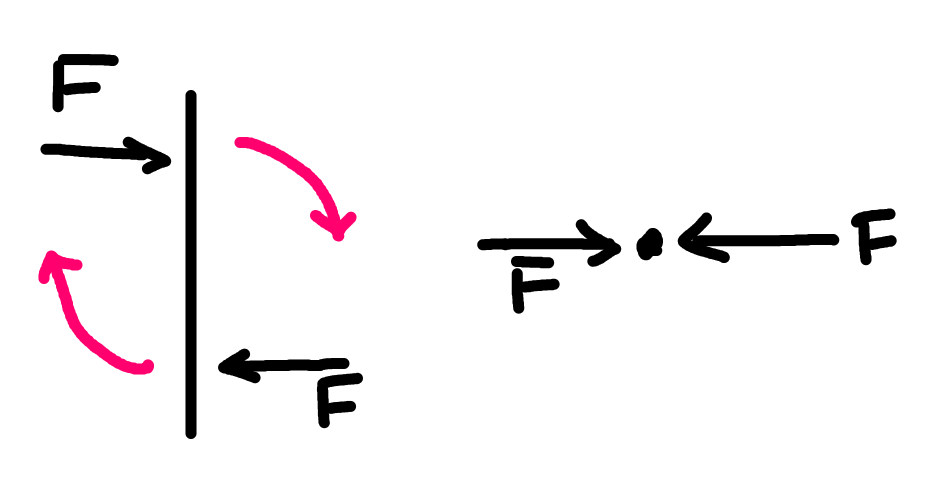
\includegraphics[width=0.5\linewidth]{notequilibrium.png}
\end{center}

Therefore, net torque $\boldsymbol{\tau}_\text{net}$ must also be $0$.

\theorem*{For an object to be in equilibrium, both net force and net torque must be zero:
\begin{equation*}
	\mathbf{F}_ \text{net}=0 \qquad \boldsymbol{\tau}_\text{net}=0
\end{equation*}}

\subsection{Stability}

\definition{A system is in \textbf{stable equilibrium} if once displaced, it experiences a net force or torque opposite to the direction of displacement, resulting in a restoring force moving it back toward the equilibrium position.}

Most systems are in stable equilibrium, especially for small displacements.

\definition{A system is in \textbf{unstable equilibrium} if once displaced, it experiences a net force or torque in the same direction of displacement. It will accelerate away from the equilibrium position even for small displacements.}

\definition{A system is in \textbf{neutral equilibrium} if its equilibrium is independent of displacement from original position. The object will remain at its new position.}

It is possible to have a combination of these situations, i.e. neutral equilibrium in one direction, but stable or unstable in another.

\subsection{Angular Acceleration}

Angular velocity $\omega$ is the rate at which the rotation angle $\theta$ changes. There is also a relationship between rotation velocity and linear velocity $v$:
\begin{equation*}
    \omega=\frac{\Delta \theta}{\Delta t}=\frac{v}{r} \qquad v=r\omega
\end{equation*}

\definition{\textbf{Angular acceleration} $\alpha$ is the rate at which angular velocity changes.
\begin{equation*}
    \alpha=\frac{\Delta\omega}{\Delta t}
\end{equation*}
where $\Delta\omega$ is the change in angular velocity and $\Delta t$ is elapsed time.}

Angular acceleration is measured in radians per second square (\si{\radian\per\second\squared}).

If $\omega\neq0$, then the object is also experiencing tangential acceleration. This is another component of the linear acceleration on the object, in addition to centripetal acceleration. Tangential acceleration is denoted $a_\text{t}$:

\begin{center}
	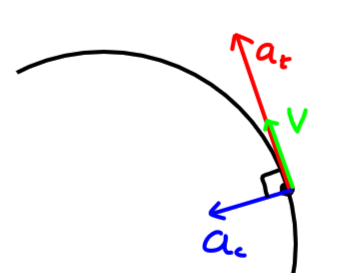
\includegraphics[width=0.3\linewidth]{circularacceleration.png}
\end{center}

Tangential acceleration is a function of angular acceleration, and $a_\text{t}=0 \iff \alpha=0$. This is unlike centripetal acceleration, which is present even if there is no angular acceleration. The magnitude of tangential acceleration $a_\text{t}=\lVert \mathbf{a}_\text{t}\rVert $ is the rate of change in the magnitude of linear velocity, denoted $\Delta v$:
\begin{align*}
	a_\text{t}&=\frac{\Delta v}{\Delta t}
	\intertext{From before, we know that linear velocity $v=r\omega$, where $r$ is the radius of rotation and $\omega$ is angular velocity:}
	a_\text{t}&=\frac{\Delta (r\omega)}{\Delta t}
\end{align*}
Since radius $r$ is constant, and by definition of angular acceleration $\alpha=\Delta \omega/\Delta t$:
\begin{equation*}
	a_\text{t}=r\alpha
	\iff \alpha=\frac{a_\text{t}}{r}
\end{equation*}

\definition{\textbf{Tangential acceleration}, or \textbf{linear acceleration}, ($\mathbf{a}_\text{t}$) is the component of an object's acceleration at any time, orthogonal to its centripetal acceleration. Its direction is the same as the object's linear velocity $\mathbf{v}$ and tangent to the circular path on which the object moves. Its magnitude is given by:
\begin{equation*}
	a_\text{t}=r\alpha
\end{equation*}
where $r$ is radius of rotation and $\alpha$ is angular acceleration (given by $\alpha=\Delta \omega/\Delta t$ where $\Delta \omega$ is change in angular velocity and $\Delta t$ is change in time).}

In fact, tangential acceleration is directly proportional to angular acceleration. Tangential acceleration affects the magnitude of the object's linear velocity, but does not affect direction of motion.

\subsection{Equations}

From linear kinematics, where $v$ is final velocity, $v_0$ is initial velocity, $t$ is time and $a$ is constant acceleration:
\begin{align*}
	v&=v_0+at
	\intertext{We know $v=r\omega$. $a$ is tangential/linear acceleration $a_\text{t}=r\alpha$.}
	r\omega&=r\omega_0+r\alpha t
	\intertext{where $\omega$ is final angular velocity and $\omega_0$ is initial angular velocity.}
	\Aboxed{\omega&=\omega_0+\alpha t}
\end{align*}

We can similarly derive other kinematic equations.

\theorem{Linear and rotational kinematics equations}{
	\begin{alignat*}{2}
		\Delta x&=\overline v\Delta t & \qquad
		\Delta\theta&=\overline\omega \Delta t \\
		\overline v&=\frac{v_0+v}{2} & \qquad
		\overline \omega&=\frac{\omega_0+\omega}{2} \\
		v&=v_0+a\Delta t & \qquad
		\omega&=\omega_0+\alpha\Delta t \\
		\Delta x&=v_0\Delta t+\frac12a(\Delta t)^2 & \qquad
		\Delta \theta&=\omega_0\Delta t+\frac12\alpha (\Delta t)^2 \\
		v^2&=v_0^2+2a\Delta x & \qquad
		\omega^2&=\omega_0^2+2\alpha\Delta \theta
	\end{alignat*}
	where:
	\begin{alignat*}{2}
		\Delta x&=\text{Change in position} & \qquad
		\Delta \theta&=\text{Change in rotation angle} \\
		v&=\text{Final linear velocity} & \qquad
		\omega&=\text{Final angular velocity} \\
		v_0&=\text{Initial linear velocity} & \qquad
		\omega_0&=\text{Initial angular velocity} \\
		\overline v&=\text{Average linear velocity} & \qquad
		\overline\omega&=\text{Average angular velocity} \\
		a&=\text{Linear acceleration} & \qquad
		\alpha&=\text{Angular acceleration} \\
		\Delta t&=\text{Elapsed time}
	\end{alignat*}
}

\section{Gravitation}

\subsection{Newton's Universal Law of Gravitation}

\theorem{Newton's universal law of gravitation}{\textbf{Newton's universal law of gravitation} states that every particle attracts every other particle with a force along the line between the two. The magnitude of the force is directly proportional to the product of the masses of the two objects and inversely proportional to the square of the distance between them. By Newton's third law, the force exerted by particle 1 on particle 2 has the same magnitude as that exerted by particle 2 on particle 1. The magnitude of the force $F$ is given by:
\begin{equation*}
    F=G \frac{mM}{r^2}
\end{equation*}
where $m,M$ are the masses of the two particles, and $r$ is the distance between their centers of mass. $G$ is the universal gravitational constant, a proportionality factor thought to be the same everywhere and experimentally determined to be approximately:
\begin{equation*}
	G\approx 6.674\times 10^{-11} \,\frac{\si{\newton\cdot\meter\squared}}{\si{\kilogram\squared}}
\end{equation*}}

The magnitude of weight/force of gravity is $F=w=mg$, where $m$ is the mass of the object. Substituting this into Newton's universal law of gravitation:
\begin{equation*}
    mg=G \frac{mM}{r^2}
	\implies 
    g=\frac{GM}{r^2}
\end{equation*}
Where $M$ is the Earth's mass and $r$ is the Earth's radius. This will show that $g\approx 9.81\,\si{\meter\per\second}$.

\subsection{Kepler's Laws of Gravitation}

We make these assumptions about orbits first:
\begin{enumerate}
	\item A small mass $m$ orbits a much larger mass $M$, such that we are able to view $M$ as stationary, and unaffected by the force of gravity exerted by $m$ upon it.
	\item The system is isolated from other masses, meaning $M$ is the only object acting on $m$.
\end{enumerate}

\definition{An object's \textbf{orbital period} is the time taken to complete one full orbit around a larger object.}

\subsubsection{Kepler's first law}

\theorem{Kepler's first law}{The orbit of each planet about a larger object is an ellipse, with the larger object at one focus of the ellipse.}

\subsubsection{Kepler's second law}

\theorem{Kepler's second law}{Each planet moves such that a sector bound by the planet's current position and the planet's position after a set amount of time is always equal, no matter the planet's current position.}

\subsubsection{Kepler's third law}

\theorem{Kepler's third law}{If $T_1,T_2$ are the periods of two orbits, and $r_1,r_2$ are the average distances from the larger object (not trivial to compute, since orbits are ellipses):
\begin{equation*}
    \frac{(T_1)^2}{(T_2)^2}=\frac{(r_1)^3}{(r_2)^3}
\end{equation*}
For a single object in a circular orbit:
\begin{equation*}
	\frac{T^2}{r^3}=\frac{4\pi^2}{GM}
\end{equation*}}

\subsubsection{Kepler's third law for circular orbits}

Consider a small mass $m$ in a circular orbit around a larger mass $M$. The small mass is in uniform circular motion. Let $r$ be the radius of curvature/the orbit, $v$ is its linear velocity, and $T$ is its orbital period. By Newton's second law, we can relate the magnitude of its centripetal acceleration $a_\text{c}$ with the magnitude of the net force exerted on the object $F_\text{net}$:
\begin{equation*}
	F_\text{net}=ma_\text{c}
\end{equation*}
We make two substitutions. First, we know that centripetal acceleration can be given in terms of linear velocity and radius: $a_\text{c}=v^2/r$. Second, there is only one force on the small mass, which is gravity from the larger mass. By Newton's law of universal gravitation, $F_\text{net}=GMm/r^2$.
\begin{equation*}
	\frac{GMm}{r^2}=\frac{mv^2}{r}
	\implies \frac{GM}{r}=v^2
\end{equation*}
The object is on a circular orbit, of length/circumference $2\pi r$, which is completed in time $T$. Hence, the magnitude of linear velocity, which remains constant, is $v=2\pi r/T$.
\begin{equation*}
	\frac{GM}{r}=\left( \frac{2\pi r}{T} \right)^2
	\implies \frac{GM}{\cancel{r}}=\frac{4\pi^2 r^2}{T^2}
	\implies T^2=\frac{4\pi^2 r^3}{GM}
\end{equation*}
Hence, we have the relationship between the orbital periods and radii of two objects.
\begin{align*}
	\Aboxed{\frac{(T_1)^2}{(T_2)^2}&=\frac{(r_1)^3}{(r_2)^3}}
	\intertext{In addition to a relationship between the mass of the larger object $M$, and the radius and orbital period of the smaller object:}
	\Aboxed{\frac{T^2}{r^3}&=\frac{4\pi^2}{GM}}
\end{align*}
(Derivation of Kepler's third law for non-circular orbits is left as an exercise to the reader.)

\section{Harmonic Motion and Oscillations}

\subsection{Hooke's Law}

\definition{\textbf{Deformation} is the displacement from an object's equilibrium position.}

\theorem{Hooke's law}{An object oscillating back and force is experiencing a force, otherwise Newton's first law implies it would continue moving in one direction. This force is known as a \textbf{restoring force}, denoted $F$.
\begin{equation*}
    F=-kx
\end{equation*}
where $k$ is the spring constant $x$ is deformation. Negative sign indicates that the restoring force is in the opposite direction of deformation.}

The potential energy stored in a spring, as stated earlier, is:
\begin{equation*}
	\text{PE}_\text{s}=\frac12kx^2
\end{equation*}

\subsection{Period and Frequency}

\definition{\textbf{Periodic motion} is motion that repeats itself at regular time intervals. The time to complete one such motion, or oscillation, is the \textbf{period} $T$. \textbf{Frequency} $f$ in periodic motion is the number of oscillations or repeated motions per unit time.}

The SI unit of frequency is a Hertz, which is an inverse second.
\begin{equation*}
	1\,\si{\hertz}
	=1\,\frac{\text{cycle}}{\si{\sec}}
	=1\,\frac{1}{\si{\sec}}
\end{equation*}

\theorem*{The relationship between frequency $f$ and period $T$ in period motion is:
\begin{equation*}
    f=\frac{1}{T}
	\implies T=\frac{1}{f}
\end{equation*}}
Then period (time) is measured in $1/\si{\hertz}=1/(1/\si{\sec})=\si{\sec}$, which makes sense.

\subsection{Simple Harmonic Motion}

\definition{\textbf{Simple harmonic motion} (SHM) describes an oscillatory motion where the system's net force is given by Hooke's law $F=-kx$. Such a system is called a \textbf{simple harmonic oscillator}. The maximum displacement from equilibrium position is the \textbf{amplitude}, denoted $X$.}

In a simple harmonic oscillator, there are no damping forces, such as friction or another nonconservative force, that reduces an object's maximum displacement from equilibrium. Hence, the local maximum of displacement to equilibrium does not change with time. This value is the amplitude $X$.

\theorem{Period and frequency of a simple harmonic oscillator}{In simple harmonic motion, the motion's frequency $f$ and period $T$ do not depend on amplitude. They are a function of the system's mass and the spring constant $k$.
\begin{equation*}
	T=2\pi \sqrt{\frac mk}
	\iff f=\frac{1}{2\pi} \sqrt{\frac km}
\end{equation*}}

The displacement of a simple harmonic oscillator at any given time is modeled by a wave:
\begin{equation*}
	x(t)=X\cos \left( \frac{2\pi t}{T} \right)
\end{equation*}
Let $v_\text{max}$ be the object's maximum velocity. At that time, it has kinetic energy $\text{KE}=\text{PE}_\text{s}$. The total spring potential energy is when displacement is at its maximum, i.e. the amplitude $X$.
\begin{equation*}
	\cancel{\frac12}mv_\text{max}^2=\cancel{\frac12}kX^2
	\implies v_\text{max}^2=\frac{kX^2}{m}
	\implies v_\text{max}=X \sqrt{\frac km}
\end{equation*}
From the above theorem, we also know that $\sqrt{k/m}=2\pi f=2\pi/T$, so we can also write $v_\text{max}$ as:
\begin{equation*}
	v_\text{max}=X \sqrt{\frac km}=2\pi f X=\frac{2\pi X}{T}
\end{equation*}
Taking the derivative of the displacement function, and applying the scaling factor $v_\text{max}$, we have the system's velocity at any time:
\begin{equation*}
	v(t)=-v_\text{max} \sin\left(\frac{2\pi t}{T}\right)
\end{equation*}
The system's maximum acceleration can be calculated from Newton's second law. From Hooke's law, the maximum force is exerted at the highest displacement (amplitude $X$), so the maximum force is $F=kX$ (no negative sign because magnitude of force is positive). Applying $F=ma$:
\begin{equation*}
	F=ma=kX
	\implies a= \frac{kX}{m}
\end{equation*}
Again, scaling the derivative of the velocity function $v$ by the maximum acceleration:
\begin{equation*}
    a(t)=-\frac{kX}{m} \cos\left(\frac{2\pi t}{T}\right)
\end{equation*}

\theorem{Position, velocity and acceleration of a simple harmonic oscillator}{The simple harmonic oscillator's position, velocity and acceleration as a function of time $t$:
\begin{align*}
	x(t)&=X \cos\left(\frac{2\pi t}{T}\right) \\
	v(t)&=-v_\text{max} \sin\left(\frac{2\pi t}{T}\right) \\
	a(t)&= -\frac{kX}{m}\cos\left(\frac{2\pi t}{T}\right)
\end{align*}
where $v_\text{max}$ is the maximum velocity obtained by the system:
\begin{equation*}
	v_\text{max}=X \sqrt{\frac km}=2\pi fX=\frac{2\pi X}{T}
\end{equation*}
where:
\begin{alignat*}{2}
	k&=\text{Spring constant} &\qquad 
	m&=\text{Mass} \\
	f&=\text{Frequency} &\qquad 
	T&=\text{Period} \\
	X&=\text{Amplitude}
\end{alignat*}}

By conservation of energy, the total energy in the system must be constant. Since we know consider kinetic energy and elastic potential energy:
\begin{align*}
	\text{KE}+\text{PE}_ \text{s}
	&=\text{constant}
	\intertext{The total energy in the system in a simple harmonic oscillator can be found by calculating the elastic potential energy in the system when the displacement is at its highest, and velocity (and therefore kinetic energy) is zero. This amount is $kX^2/2$. At any displacement from the equilibrium (deformation) $x$, we know kinetic energy and spring potential energy:}
	\frac12mv^2+\frac12kx^2&=\frac12kX^2
\end{align*}
where $m$ is the system's mass, $k$ is the spring constant, $X$ is amplitude, $x$ is current deformation and $v$ is current velocity. Solving for velocity $v$:
\begin{equation*}
    v=\pm\sqrt{\frac{kX^2-kx^2}{m}}
	=\pm \sqrt{\frac km}\sqrt{X^2 \left( 1-\frac{x^2}{X^2} \right)}
	=\pm \left( X \sqrt{\frac km} \right) \sqrt{1-\frac{x^2}{X^2}}
\end{equation*}
Notice that the maximum velocity $v_\text{max}=X \sqrt{k/m}$. Substituting:
\begin{equation*}
	\boxed{v=\pm v_\text{max} \sqrt{1-\frac{x^2}{X^2}}}
\end{equation*}
Actually, this is the same as the formula for velocity stated earlier. If we take the position $x=X \cos\left(2\pi t/T\right)$:
\begin{equation*}
	v
	=\pm v_\text{max} \sqrt{1-\frac{X^2\cos^2 \left( 2\pi t/T \right)}{X^2}}
	=\pm v_\text{max} \sqrt{1-\cos^2 \left( 2\pi t/T \right)}
	=\pm v_\text{max} \left| \sin\left(\frac{2\pi t}{T} \right)\right|
	=-v_\text{max} \sin\left(\frac{2\pi t}{T}\right)
\end{equation*}
$\pm$ and absolute value become just a negative sign to indicate the velocity is in the opposite direction of displacement. If that sounds like hand-waving we can simply apply ``\textit{proof by convenience}.''

\subsection{Simple Pendulum}

\definition{A \textbf{simple pendulum} is an object with a small mass, known as the \textbf{pendulum bob}, suspended by a string or wire to a pivot point.}

\begin{center}
	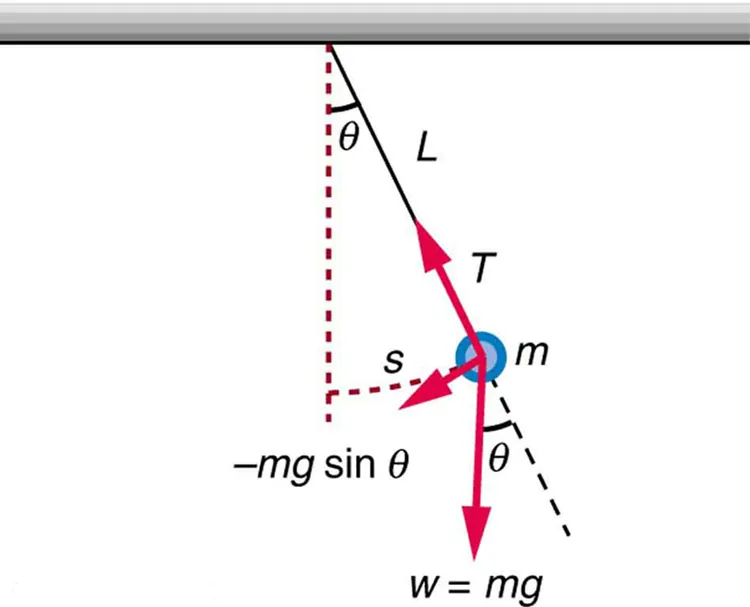
\includegraphics[width=0.5\linewidth]{pendulum.png}
\end{center}

The above pendulum is angle $\theta$ away from its equilibrium position, and its displacement from equilibrium is the arc length $L\theta$, where $L$ is the constant displacement between the mass and the pivot point.

There is a force of gravity upon the pendulum bob of magnitude $w=mg$. Weight has two components, one of which is in the direction towards the pivot point from the bob ($mg\sin\theta$), and a restoring force which is tangent to the arc:
\begin{equation*}
    F=-mg \sin\theta
\end{equation*}
where $F$ is the restoring force tangent to the arc causing the bob to to swing, $m$ is the mass of the bob and $g$ is the gravitational constant. The negative sign indicates the force is opposite to displacement from equilibrium.

For small angles $\theta$, we can use the small angle approximation $\sin\theta\approx\theta$. Since $s$ is the arc length with $s=L\theta\implies \theta=s/L$:
\begin{equation*}
    F=-mg\theta
	\implies F=-\frac{mg}{L}s
\end{equation*}
which is Hooke's law with the spring constant $k=mg/L$. Hence, for simple pendulums with a small angle ($\theta<15^\circ$), we can use equations for simple harmonic motion derived in the previous section, with $k=mg/L$. For example, the amplitude of a pendulum with small angle:
\begin{equation*}
    T
	=2\pi \sqrt{\frac mk}
	=2\pi \sqrt{\frac{\cancel{m}}{\cancel{m}g/L}}
	=2\pi \sqrt{\frac Lg}
\end{equation*}


\end{document}
